\documentclass[12pt,floatfix,showpacs]{revtex4-1}

\usepackage{amssymb,amsmath,amsfonts}
\usepackage{graphicx}

\newcommand{\eg}{\emph{e.g., }}
\newcommand{\ie}{\emph{i.e., }}
\newcommand{\etal}{\emph{et al.}}

% remove these for final publication 
\usepackage{color} 
\newcommand{\note}[1]{\textcolor{red}{#1}}
\newcommand{\gnote}[1]{\marginpar{\textcolor{red}{\scriptsize{#1}}}}

\graphicspath{{./graphics/}{./pdfgraphics/}}  % remove pdfgraphics path for final publication!

\begin{document}

\title{Stability and Edge-Localized Mode Characterization in I-Mode Pedestals}

\author{JR Walk}
\email[]{jrwalk@psfc.mit.edu}
\affiliation{MIT Plasma Science and Fusion Center}

\author{JW Hughes}
\affiliation{MIT Plasma Science and Fusion Center}

\author{PB Snyder}
\affiliation{General Atomics}

\author{AE Hubbard}
\affiliation{MIT Plasma Science and Fusion Center}

\author{B LaBombard}
\affiliation{MIT Plasma Science and Fusion Center}

\author{DF Brunner}
\affiliation{MIT Plasma Science and Fusion Center}

\author{JL Terry}
\affiliation{MIT Plasma Science and Fusion Center}

\author{DG Whyte}
\affiliation{MIT Plasma Science and Fusion Center}

\author{AE White}
\affiliation{MIT Plasma Science and Fusion Center}

\author{E Edlund}
\affiliation{Princeton Plasma Physics Laboratory}

\date{\today}

\begin{abstract}
I-mode is a novel high-confinement tokamak regime characterized by H-mode-like enhanced energy confinement and the formation of a strong temperature pedestal, without the accompanying density pedestal or enhanced particle confinement, maintaining an L-mode-like density profile.  I-mode exhibits a number of desirable properties for a reactor regime, including a lack of strong degradation of energy confinement with heating power and apparent naturally-occurring suppression of large ELMs, avoiding the need for externally-applied ELM suppression.  However, under certain conditions (particularly, reduced toroidal field) small, intermittent ELM-like events are seen, although these cases are modeled to be stable to the peeling-ballooning MHD instability associated with the ELM trigger, as is typical of I-mode pedestals.  We examine these events in detail to better characterize the edge stability behavior in I-mode.  The majority of observed ELM candidates are observed to be synchronized with the sawtooth heat pulse reaching the pedestal, which measurably perturbs the temperature pedestal.  However, this perturbation appears to be insufficient to reach the peeling-ballooning stability boundary; moreover, the ELM candidate does not include a ``crash'' in the pedestal temperature or stored energy.  \note{precursor fluctuations?  include Ahmed?  Ref divertor heat flux measurements?}  In short, these events do not appear to be true instability-driven ELMs, but rather are benign $H_\alpha$ spikes driven by the sawtooth heat pulse.  A minority of the ELM candidates in I-mode do include the characteristic temperature crash associated with an ELM, and are not necessarily sawtooth-triggered -- however, these events are isolated, and the stationary pedestal structure in these I-modes is also modeled to be stable to the ELM trigger, indicating that transient events in the pedestal drive these ELMs, rather than an inherent instability of the pedestal.
\end{abstract}

\pacs{52.55.Fa, 52.55.Tn, 52.35.Py, 52.25.Fi, 52.40.Hf}

\maketitle

%%%%%%%%%%%%%%%%%%%%%%%%%%%%%%%%%%%%%%%%%%%%%%%%%%%%%%

\section{Introduction}\label{sec:intro}

The development of tokamak magnetic-confinement fusion into a viable \& economical form of power generation faces two overarching (and seemingly contradictory) requirements.  
First, a high level of energy confinement is necessary for net energy production with the desired level of self-heating of the plasma by fusion products.  
At the same time, sufficient particle transport is needed to avoid the deleterious effects of accumulated impurities (both helium ``fusion ash'' and higher-$Z$ impurities from the erosion of plasma-facing components) due to fuel dilution and radiative losses.  
This has been achieved in a number of operating regimes, collectively termed ``high-confinement'' or H-modes \cite{Wagner1982}.  

H-modes are characterized by a steep gradient region at the plasma edge in density, temperature, and pressure, termed the \emph{pedestal}, the height of which is strongly correlated with global fusion performance \cite{Kinsey2011}.  
These strong gradients have been shown to drive edge MHD instabilities \cite{Huysmans2005,Maget2013,Snyder2002} resulting in an Edge-Localized Mode (ELM), an explosive perturbation to the pedestal expelling energy and particles into the plasma exhaust \cite{Zohm1996}.  
On existing experiments, ELMs drive sufficient particle transport to allow stationary operation with acceptable radiative losses \cite{Keilhacker1984}; as ELMy H-modes are robust and straightforward to achieve, this regime is considered the baseline for ITER operation \cite{ITER1999,Shimada2007}.  
However, on ITER-scale devices ELMs drive transient heat loads to the divertor, leading to unacceptable levels of erosion and damage to plasma-facing components \cite{Loarte2003,Federici2003}.
This introduces an additional requirement for tokamak fusion reactor concepts -- the avoidance, suppression, or mitigation of large ELMs, either via externally-applied engineering solutions (pellet pacing \cite{Baylor2013,Lang2014} or resonant magnetic perturbations \cite{Evans2004,Evans2006}), or via alternate high-confinement regimes which regulate the pedestal below the ELM limit (\eg the Enhanced $D_\alpha$ (EDA) H-mode \cite{Greenwald1999,Hubbard2001} or the QH-mode \cite{Burrell2002,Suttrop2005}).

The I-mode \cite{Whyte2010,Walk2014,Walk2014b}, pioneered on the Alcator C-Mod tokamak \cite{Hutchinson1994}, is one such alternate regime for high-performance operation.

\begin{figure}[ht]
 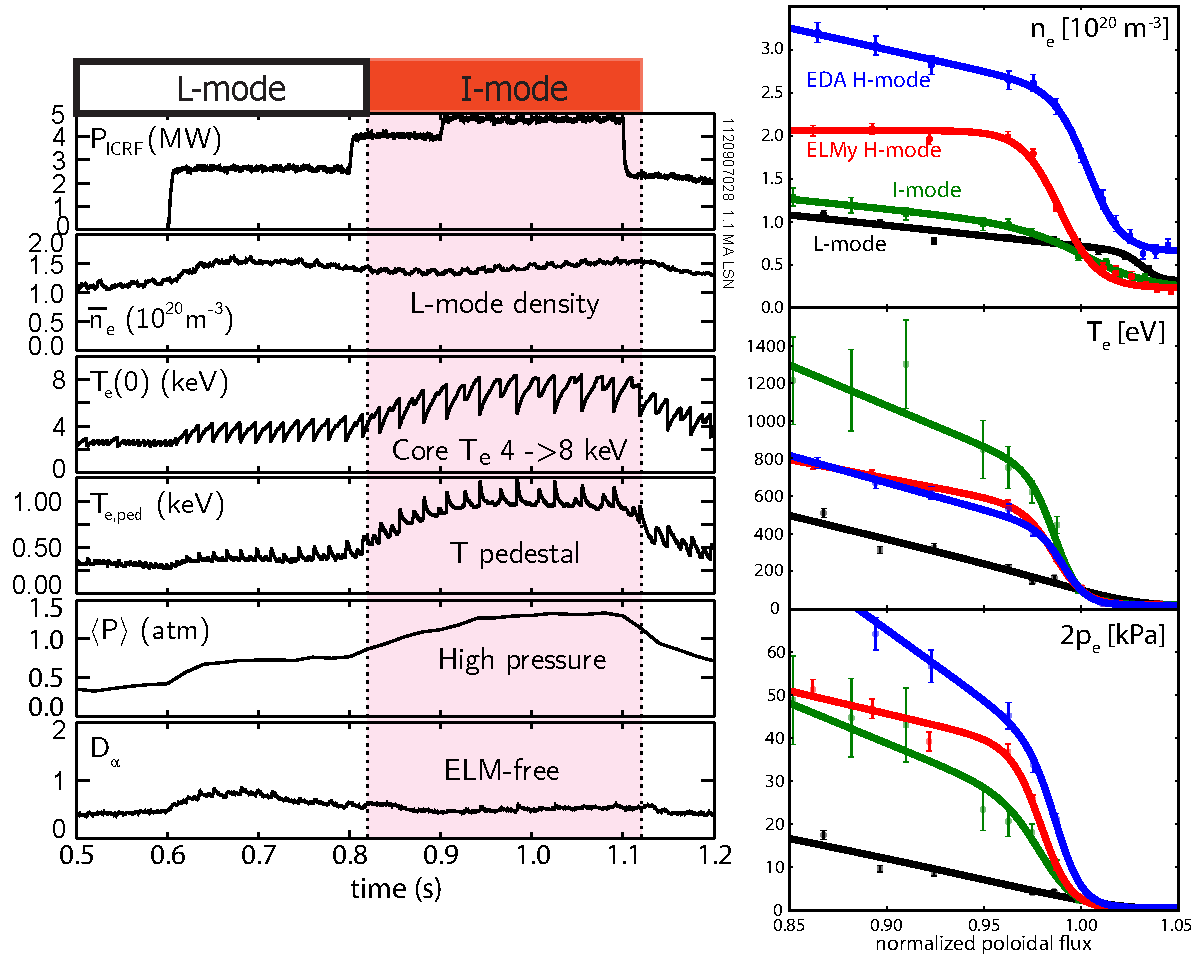
\includegraphics[width=\textwidth]{trace_imode.pdf}
 \caption{(left) characteristic time traces for an I-mode.  After the L-I transition, the core and edge temperature rise over several sawtooth cycles (visible in the oscillations in $T_e(0)$ and $T_{e,ped}$) before reaching a steady level; global pressure and confinement rise accordingly.  However, the density remains unchanged from the L-mode level.  No ELMs are exhibited on the $D_\alpha$ trace.  (right) pedestal profiles for L-, I-, and H-modes.  The I-mode (green) retains a density profile similar to L-mode (black), unlike the ELMy (red) and EDA (blue) H-modes, which form a strong density pedestal.  However, the I-mode forms a higher temperature pedestal than either H-mode, resulting in comparable pedestal pressures to H-mode while retaining L-mode particle transport.}
 \label{fig:imode_trace}
\end{figure}

%%%%%%%%%%%%%%%%%%%%%%%%%%%%%%%%%%%%%%%%%%%%%%%%%%%%%%

\begin{acknowledgments}
 Experimental work on Alcator C-Mod is supported by US DOE agreement DE-FC02-99ER54512. Theory work at General Atomics is supported by US DOE agreement DE-FG02-99ER54309.  The authors also wish to acknowledge the efforts of the Alcator C-Mod team for supporting the experiments reported here.
\end{acknowledgments}

% remove \bibliography call, paste in bbl file
% actually, peerx-press says they accept bib files now!
% construct proper bib file once citations are all put together
\bibliographystyle{aipnum4-1}
\bibliography{jrwalk_references}

\end{document}